\chapter{Testes de Verificação e Validação}

%\section{Características Gerais}

%\textcolor{red}{Introduzir os principais pontos deste capítulo. Cada teste deve %conter explicações completas que garantam sua repetibilidade:
% \begin{itemize}
%     \item Hipóteses levantadas
%     \item Condições de contorno
%     \item Resultados esperados
%     \item Materiais e métodos
%     \item Precisão e acurácia das medidas obtidas.
% \end{itemize}
%}

\section{Testes da estrutura}

Testes sobre a estrutura e versões dos protótipos do chassi e labirinto.

\subsection { Testes Estrutura e Prototipagem do Micromouse}

Para o refinamento da estrutura do Micromouse, foram fabricados por impressão 3D, utilizando materiais PETG e PLA, três versões do chassi, duas versões da tampa do compartimento da bateria e dois suportes de fixação, conforme apresentado nas Figuras~\ref{fig:prot_chassis}, \ref{fig:prot_chassis_angulo} e \ref{fig:prot_versao_final}.


\begin{figure}[htbp]
\centering
\begin{minipage}{.5\textwidth}
  \centering
  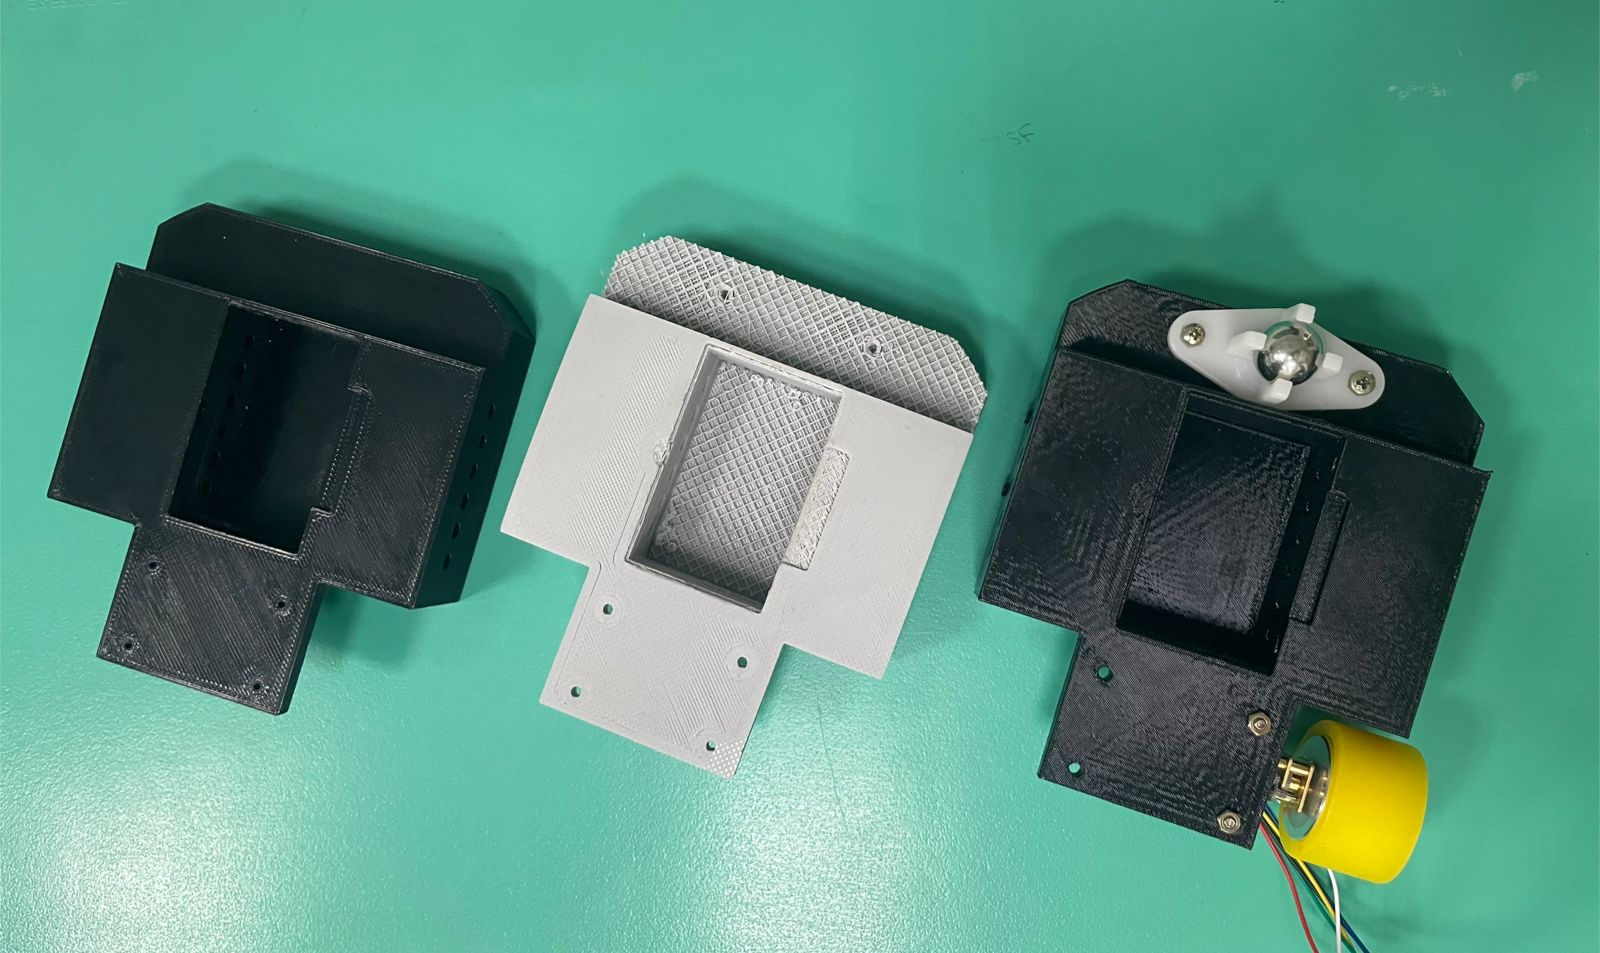
\includegraphics[width=0.7\textwidth]{figuras/versoes_chassi.jpeg}
  \captionof{figure}{Protótipos fabricados por impressão 3D.}
  \label{fig:prot_chassis}
\end{minipage}%
\begin{minipage}{.5\textwidth}
  \centering
  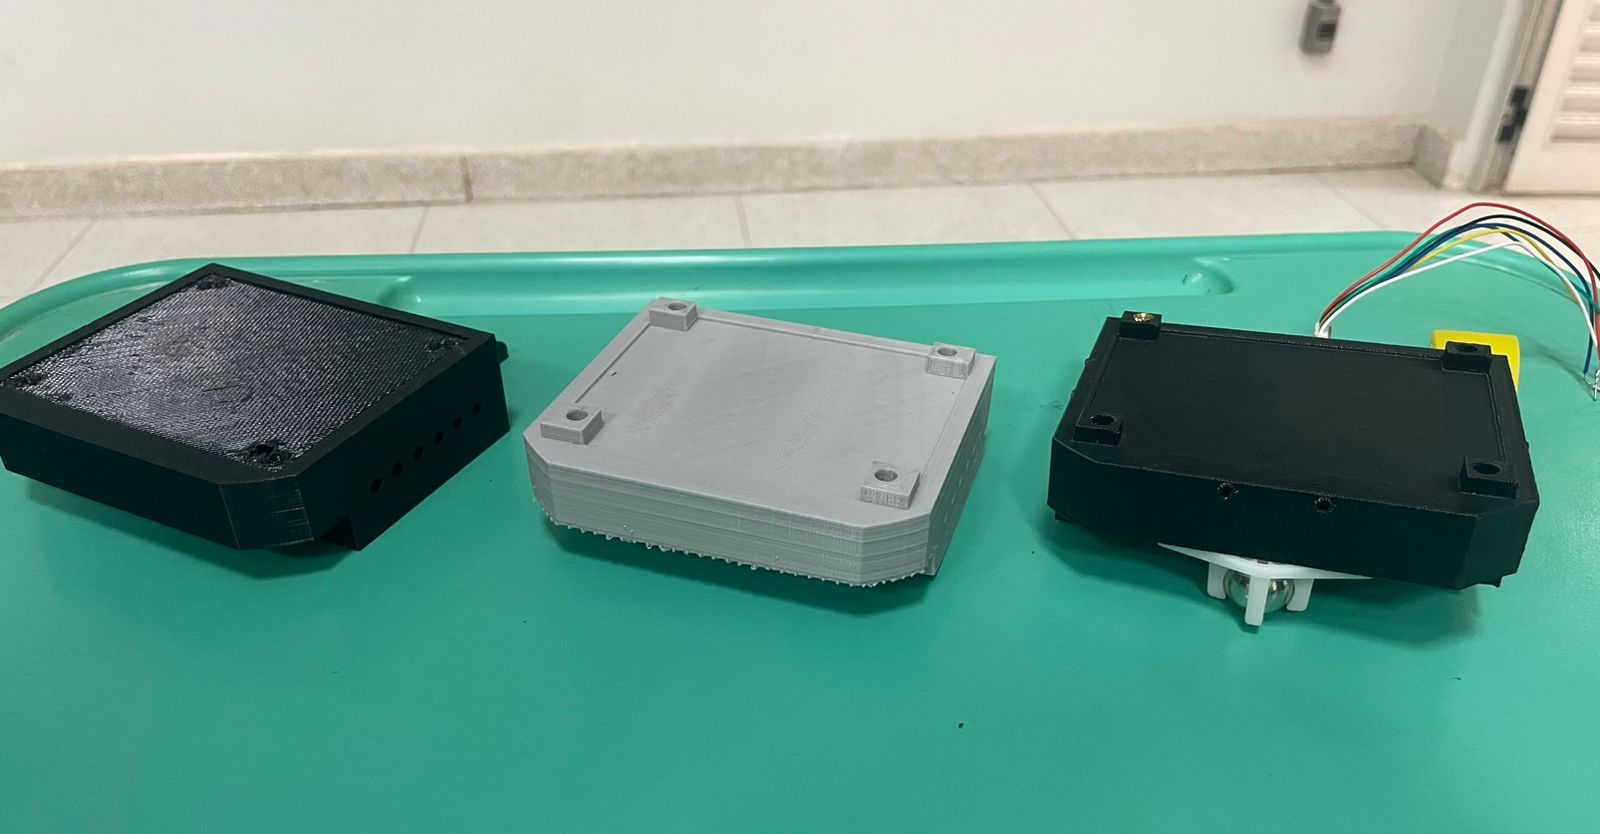
\includegraphics[width=0.7\textwidth]{figuras/versoes_chassi_angulo.jpeg}
  \captionof{figure}{Outro ângulo.}
  \label{fig:prot_chassis_angulo}
\end{minipage}
\end{figure}


Entre o projeto conceitual e a versão final, foram realizadas as seguintes modificações: ajuste dos diâmetros dos furos para compatibilidade com insertos metálicos comerciais; inclusão de ressaltos na base do sistema eletrônico para evitar interferências com componentes e pontos de solda localizados na face inferior da placa eletrônica; alteração do sistema de encaixe da tampa e reposicionamento da saída de fiação, proporcionando melhor acomodação dos cabos; realocação dos sensores ToF das laterais da placa eletrônica para as faces externas do chassi.

Essas alterações resultaram em uma melhor integração entre os componentes do sistema, contribuindo para maior robustez estrutural e facilidade de montagem.

\begin{figure}[H]
   \centering
   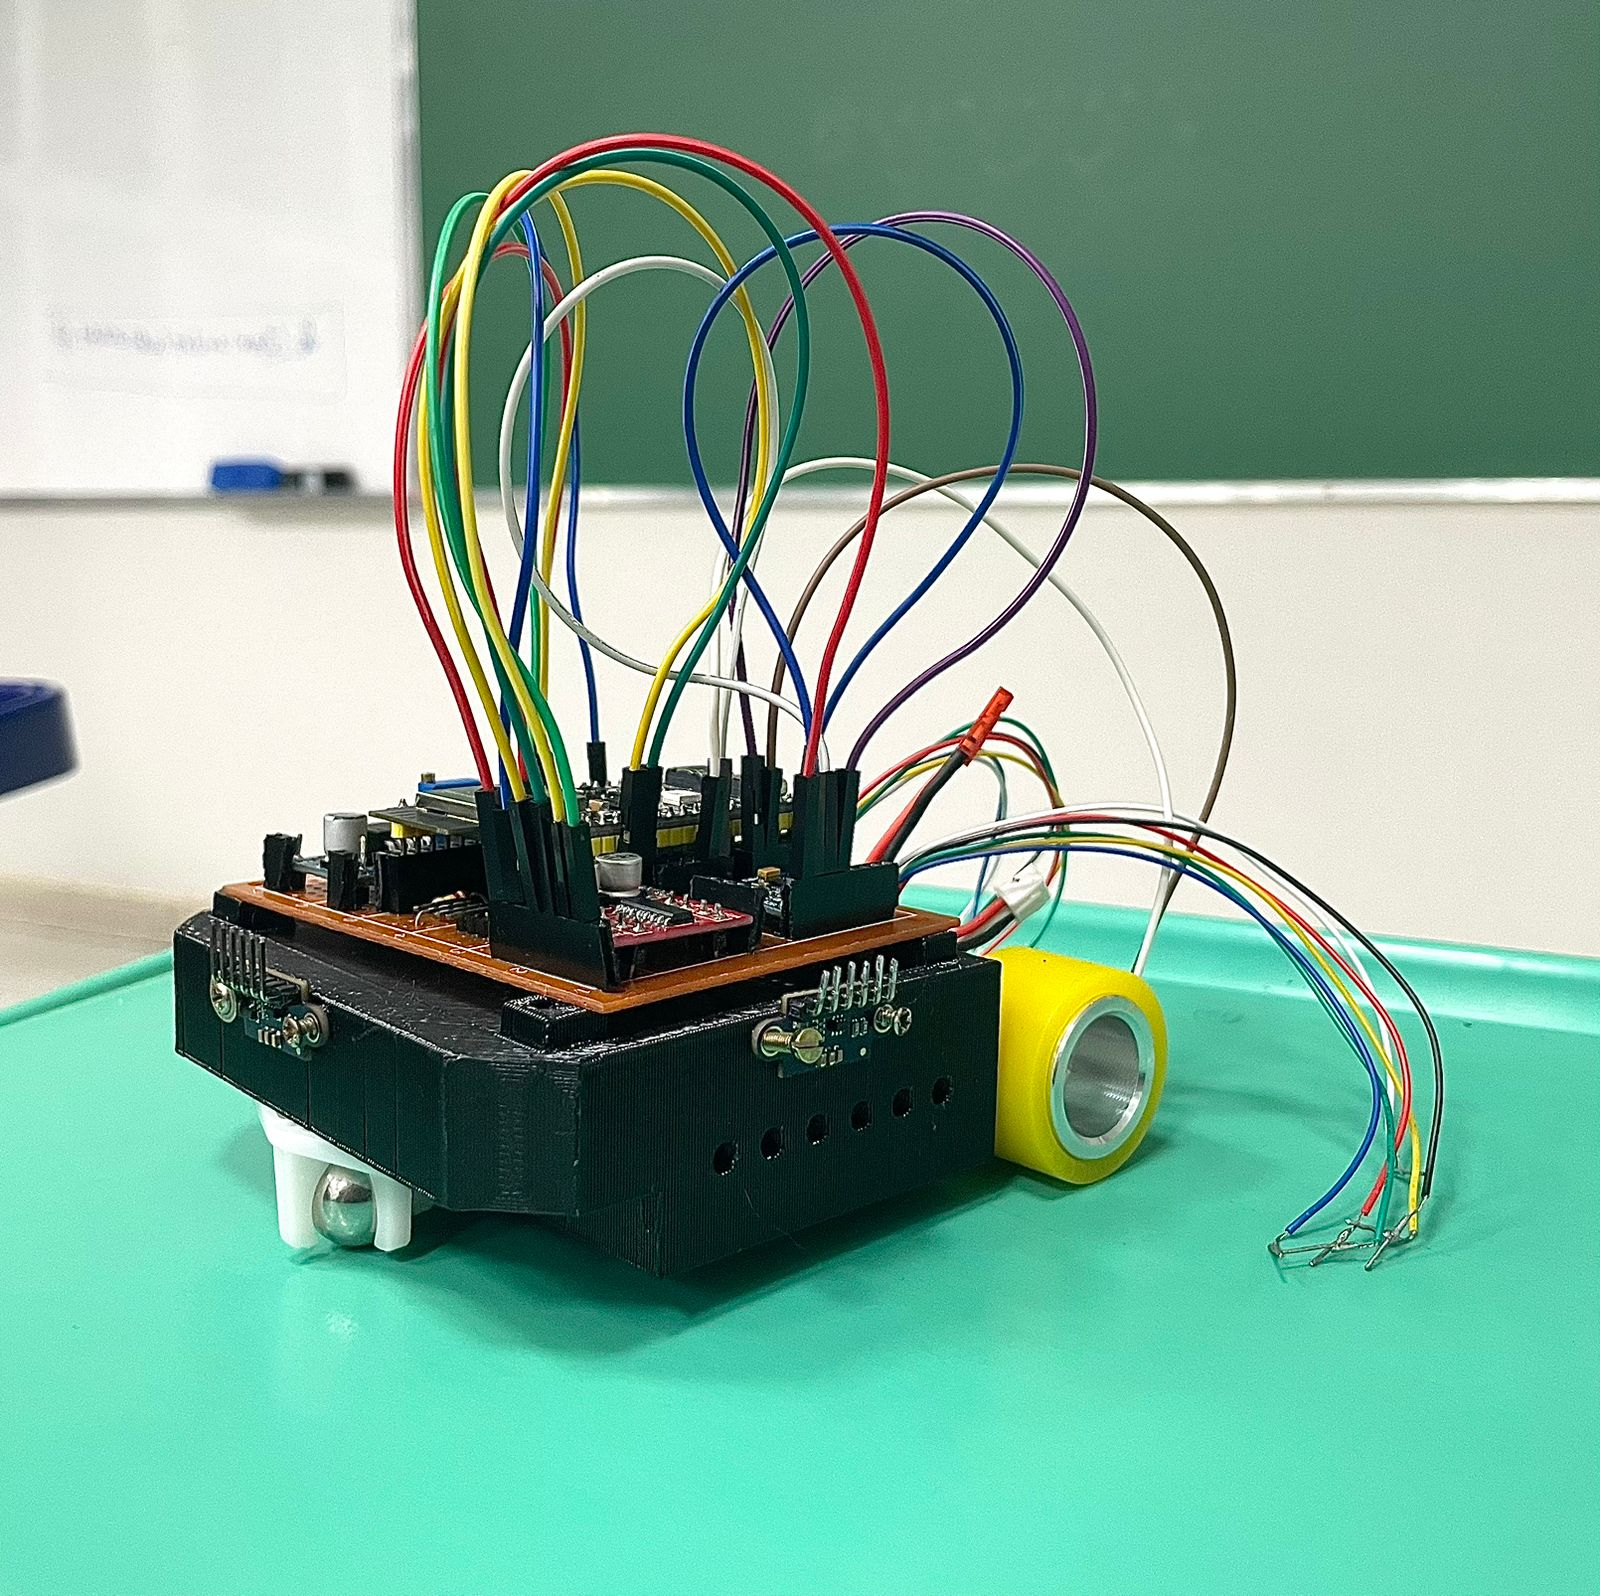
\includegraphics[width=0.45\textwidth]{figuras/versao1.2.jpeg}
   \caption{Protótipo da versão 1.2 por impressão 3D.}
   \label{fig:prot_versao_final}
\end{figure}

%\begin{figure}[H]
   % \centering
   % \includegraphics[width=0.7\textwidth]{montagem_final.jpg}
   % \caption{Montagem final do sistema Micromouse.}
   % \label{fig:montagem_final}
%\end{figure}

\subsection {Testes do labirinto}


Após a realização dos cálculos preliminares, modelagem em CAD e realização do desenho
técnico do labirinto, foi iniciada sua fabricação. As chapas de MDF foram adquiridas em
dimensões maiores do que as necessárias, sendo preciso realizar cortes para que elas se
adequassem às medidas definidas no projeto.


Durante a montagem, foi identificado um erro no dimensionamento das laterais do labirinto,
onde o cálculo inicial considerou uma parede a menos do que o necessário, resultando em
células com dimensões diferentes entre si tal como evidenciado nas Figuras~\ref{fig:montagemlabirintov1.0} e \ref{fig:labirinto}. Para corrigir o problema, optou-se por reajustar
as dimensões totais do labirinto, de modo que as paredes internas passassem a compor a
medida prevista de 18 x 18 cm para cada célula. Com essa alteração, as dimensões
externas do labirinto foram reduzidas para 72 x 72 cm. As paredes mantiveram a espessura
de 1,5 cm, conforme definido no projeto conceitual, enquanto a dimensão interna de cada
uma das 16 células passou a ser 16,125 x 16,125 cm. Dessa forma, como consta na Figura~\ref{fig:montagemlabirintov1.1}, o labirinto tornou-se
mais compacto, mas continuou atendendo aos requisitos estabelecidos para os testes.

\section{Testes de \textit{hardware}}

Seção para relato dos testes de hardware, que incluem testes de processamento, sensores, armazenamento, atuadores e comunicações.

\subsection{ESP32}
\subsubsection{\textit{Dual Core}}
Para validar o funcionamento da ESP32 e de seus dois núcleos de processamento, foi realizado um teste utilizando o FreeRTOS. A execução das tarefas foi monitorada por meio da comunicação serial, permitindo verificar a correta operação dos dois núcleos do microcontrolador. 

Foi desenvolvida uma rotina simples em que duas tarefas independentes eram atribuídas a núcleos distintos da ESP32. Cada tarefa enviava uma mensagem pela interface serial contendo a identificação do núcleo responsável pela execução. O resultado do teste é apresentado na Figura \ref{fig:teste_dualcore}. 

\subsubsection{Comunicação}
Para validar a comunicação Wi-Fi da ESP32, foi desenvolvido um algoritmo simples de conexão à rede. Durante o teste, utilizou-se uma rede Wi-Fi pessoal, cujos dados de identificação foram omitidos para preservar a privacidade dos integrantes da equipe.

Após o estabelecimento da conexão, foi realizada uma requisição HTTP ao endereço \href{http://jsonplaceholder.typicode.com/posts/1}{http://jsonplaceholder.typicode.com/posts/1}, seguida da leitura dos dados retornados pelo servidor. Após duas requisições bem-sucedidas, a conexão com a internet foi interrompida com o objetivo de verificar o comportamento do sistema e as mensagens de erro geradas na ausência de conectividade.

A Figura \ref{fig:teste_Wifi} exibe uma captura do monitor serial contendo as informações transmitidas durante o teste.

\subsection{Sensores}
\subsubsection{TOF}
Para validar os sensores TOF, foram coletados dados de distância considerando os limites estimados para a detecção de obstáculos pelo veículo. As medições foram feitas com um objeto branco fixo em frente ao sensor e as distâncias de referência adotadas foram de 80mm para o limite lateral e 50mm para o limite frontal. Durante a coleta, a posição do sensor foi mantida fixa e ajustada com o auxilio de uma régua milimetrada. Foram obtidas 403 amostras para o limite lateral e 334 amostras para o limite frontal, ambas com frequência de amostragem de 4Hz. A analise estatística dos dados coletados é apresentada na Tabela \ref{tab:tof_stats}. 

\begin{table}[h]
    \centering
       \begin{tabular}{|l|c|c|}
        \hline
        \textbf{Distância} & \textbf{Limite Lateral} & \textbf{Limite Frontal} \\ \hline
        
        \multicolumn{3}{|c|}{\textbf{Dados Gerais}} \\ \hline
        Amostras originais & 403 & 334 \\ \hline
        Outliers removidos & 0 & 1 \\ \hline
        Amostras utilizadas & 403 & 333 \\ \hline
        
        \multicolumn{3}{|c|}{\textbf{Medidas de Tendência}} \\ \hline
        Média & 81,422 & 50,928 \\ \hline
        Mediana & 81,000 & 51,000 \\ \hline
        
        \multicolumn{3}{|c|}{\textbf{Medidas de Dispersão}} \\ \hline
        Desvio padrão & 2,031 & 3,320 \\ \hline
        Coeficiente de variação (CV) & 2,494\% & 6,520\% \\ \hline
        
        \multicolumn{3}{|c|}{\textbf{Extremos}} \\ \hline
        Mínimo & 76,000 & 43,000 \\ \hline
        Máximo & 87,000 & 59,000 \\ \hline
        
        \multicolumn{3}{|c|}{\textbf{Quartis}} \\ \hline
        Q1 & 80,000 & 48,750 \\ \hline
        Q3 & 83,000 & 53,000 \\ \hline
    \end{tabular}
    \caption{Análise estatística das medições do sensor TOF para os limites lateral e frontal.}
    \label{tab:tof_stats}
\end{table}

Durante os testes, também foi observado que a distância entre os sensores e a superfície sobre a qual o micromouse navegará influencia a precisão das medições. Em alturas reduzidas, as leituras apresentaram rápido aumento de imprecisão, tendendo a valores inferiores às distâncias reais. Essa observação indica que o posicionamento dos sensores deve ser considerado durante o projeto mecânico do veículo. Registros desse comportamento podem ser encontrados nas demonstrações disponíveis no \href{https://unbbr-my.sharepoint.com/:v:/g/personal/231027079_aluno_unb_br/IQD2xGlDyRQrT7hCBopCS1RXAX4SP_C7y0wbpGJBctz3md8?nav=eyJyZWZlcnJhbEluZm8iOnsicmVmZXJyYWxBcHAiOiJPbmVEcml2ZUZvckJ1c2luZXNzIiwicmVmZXJyYWxBcHBQbGF0Zm9ybSI6IldlYiIsInJlZmVycmFsTW9kZSI6InZpZXciLCJyZWZlcnJhbFZpZXciOiJNeUZpbGVzTGlua0NvcHkifX0&e=rYLxsI}{OneDrive do projeto}. 

A partir dos dados analisados, observa-se que as leituras apresentam boa estabilidade, com pequenas variações em torno das distâncias de referência. Deve-se ressaltar que o método de posicionamento adotado introduz uma parcela de erro fixo nas medições, associada ao alinhamento manual do sensor e do objeto durante os testes. Considerando os resultados obtidos, os dados sugerem que o sensor ToF é adequado para a detecção das paredes do labirinto nas distâncias avaliadas. 

\subsubsection{MPU 6050}
Para calibração da MPU 6050, foram utilizados dois métodos: a obtenção, via média de erro de leitura, de valores de offset para cada eixo de cada sensor, e a implementação do filtro passa-baixa configurável existente no módulo via biblioteca nativa \emph{Adafruit\_MPU6050.h}. O sensor foi mantido ligado e coletou quantidades satisfatórias de dados sob as duas condições (antes e depois da calibração). Os resultados foram documentados e comparados, a fim de determinar a aplicabilidade da filtragem e frequência escolhida e dos parâmetros de offset obtidos numericamente. Os resultados das medições podem ser observados a partir dos gráficos \ref{fig:fft_acelerometro_x} a \ref{fig:fft_giroscopio_z} e da tabela \ref{tab:calibracao_mpu}.

\begin{table}[htbp]
\centering
\caption{Desvio padrão médio, mínimos e máximos em cada eixo obtidos em leitura dos dados da MPU 6050 antes e depois da aplicação dos métodos de calibração.}
\label{tab:calibracao_mpu}
\renewcommand{\arraystretch}{1.5} 
\begin{tabular}{|p{2.5cm}|p{2.8cm}|p{2.8cm}|p{2.8cm}|p{2.8cm}|}
\hline
 & \textbf{Acelerômetro (dados brutos)} & \textbf{Acelerômetro (dados tratados)} & \textbf{Giroscópio (dados brutos)} & \textbf{Giroscópio (dados tratados)} \\ \hline
\textbf{SD médio entre eixos} & 0.06827 & 0.00816 & 0.02462 & 0.00311 \\ \hline
\textbf{X mín.} & 0.59 & -0.10 & -1.17 & 0.00 \\ \hline
\textbf{Y mín.} & -1.62 & 0.02 & -0.94 & -0.01 \\ \hline
\textbf{Z mín.} & 5.19 & 9.78 & -0.41 & -0.01 \\ \hline
\textbf{X máx.} & 4.49 & 0.06 & 3.02 & 0.00 \\ \hline
\textbf{Y máx.} & 1.10 & 0.09 & 2.92 & 0.00 \\ \hline
\textbf{Z máx.} & 16.8 & 9.86 & 0.13 & 0.01 \\ \hline
\end{tabular}
\end{table}

Os dados foram coletados com o sensor parado e posicionado na horizontal, paralelo ao chão. Foi utilizada uma frequência de amostragem de 50 Hz. Os dados sem o filtro foram coletados por um tempo aproximado de 3 minutos e 19 segundos, totalizando 9950 amostras. Com o filtro passa-baixa habilitado e configurado para a frequência de 5 Hz através da função \emph{mpu.setFilterBandwidth} e o offset calculado aplicado em todos os eixos, foram coletadas um total de 6554 amostras, em um tempo aproximado de 2 minutos e 12 segundos. 

Ao analisar os gráficos e a tabela, nota-se que os dados de máximos e mínimos pós filtragem e aplicação de offset mostram-se mais concisos e coerentes com o posicionamento do sensor, pois espera-se, a partir da configuração descrita anteriormente, valores próximos de 0 em todos os eixos do giroscópio. Quanto ao acelerômetro, são esperados valores próximos de 0 em todos os eixos, com exceção do eixo Z, que, por conta da leitura da aceleração da gravidade, deve apresentar valores próximos a 9.8. Observa-se, também, uma diminuição considerável nas amplitudes e nos picos em bandas de frequência isoladas das amostras filtradas quando comparadas às amostras não filtradas. A diminuição dessa inconsistência resultou em um desvio padrão médio entre os três eixos substancialmente menor no sampling filtrado tanto no acelerômetro quanto no giroscópio, como demonstrado pela tabela \ref{tab:calibracao_mpu}. 

Os dados amostrados indicam que a aplicação dos métodos de calibração escolhidos resultaram em uma melhora significativa na confiabilidade, precisão e consistência dos dados de output da MPU 6050.

\subsubsection{Regulador de tensão e porcentagem de carga da bateria}
Para garantir uma alimentação adequada da ESP32, foi utilizado um regulador de tensão ajustável. Com o auxílio de um multímetro e da bateria prevista para o projeto, a tensão de saída foi ajustada para 5 V por meio de um trimpot, considerando a utilização do regulador interno da ESP32 DevKit. O resultado do ajuste é apresentado na Figura \ref{fig:regulador_tensao}.

Para identificar a porcentagem de carga disponível na bateria, foi utilizado um divisor de tensão conectado à entrada analógica da ESP32. O circuito também inclui um capacitor de desacoplamento, responsável pela filtragem de ruídos e pela estabilização do sinal medido. O sistema foi validado utilizando um multímetro e uma fonte de tensão contínua ajustável, permitindo observar a resposta do circuito para diferentes níveis de tensão dentro da faixa de operação prevista para a bateria do projeto. O resultado da validação é apresentada na figura \ref{fig:medidor_tensao}. 


\subsection{Atuadores}
\subsubsection{Ponte H L298N e motores DC 6V}
Uma vez que a ponte H e os motores DC 6V funcionam juntos, optou-se por realizar testes em ambos como conjunto, e não de cada um dos componentes separadamente. Os testes foram realizados via firmware com controle periódico de PWM e sentido de rotação, gravado na ESP32 conectada à ponte H. A alimentação da L298N foi feita a partir dos pinos de alimentação do devkit do microcontrolador. Os terminais de alimentação dos motores foram conectados diretamente aos terminais da bateria. 

O sistema apresentou o comportamento esperado em todas as etapas de teste. As variações de PWM, em intervalos de 50 (o argumento do PWM varia de 0 a 255), resultaram em mudanças na velocidade do motor. A mudança nos bits de sentido resultou em alteração no sentido de rotação, que, no firmware utilizado no teste, mudou a cada 2 segundos. Ambos os canais da ponte H e ambos os motores DC foram testados e avaliados, com resultados semelhantes obtidos em todos os cenários testados. Devido ao caráter qualitativo do protocolo de teste desse sistema, parte do teste foi registrado em formato de vídeo, que pode ser acessado através \href{https://unbbr-my.sharepoint.com/:f:/g/personal/231027079_aluno_unb_br/IgBTkERhmse0RpFUGiqooULzAQvzFr9VL5YGq6soeIDkyNI?e=624aZd}{deste link}.

\section{Testes de consumo energético}

Para a validação prática do dimensionamento energético, foi realizado um teste experimental com o protótipo operando pelo tempo de 20 minutos (1200 segundos). A metodologia consistiu de 10 medições de tensão ($V_k$) e corrente ($I_k$) em intervalos regulares ao longo do percurso. A partir de cada par de dados coletados, determinou-se a potência instantânea por meio do produto $P_k = V_k \cdot I_k$, gerando 10 valores distintos de potência. Na sequência, calculou-se a potência média operacional ($\bar{P}$) através da média aritmética simples dessas amostras. Por fim, esse valor médio de 15,58 W foi multiplicado pelo tempo total de operação convertido para horas ($1200/3600$ h) para a determinação da potência final consumida de 5,19 Wh. A Tabela \ref{tab:comparativo_eletrico} apresenta o comparativo entre os dados projetados no modelo teórico ideal e os dados medidos durante a validação.

\begin{table}[h!]
\centering
\caption{Comparativo de Parâmetros Elétricos (Teórico vs. Real)}
\label{tab:comparativo_eletrico}
\renewcommand{\arraystretch}{1.3}
\begin{tabular}{lcc}
\hline
\textbf{Parâmetro} & \textbf{Modelo Teórico} & \textbf{Teste Real} \\ \hline
Tensão Média Operacional & 7,40 V & 7,60 V \\ 
Potência Média & 14,15 W & 15,58 W \\ 
Energia Consumida (20 min) & 4,71 Wh & 5,19 Wh \\ 
Condição Final da Bateria & -- & 7,22 V \\ \hline
\end{tabular}
\end{table}

A bateria começou o teste com sua carga máxima de 8,4 V (tensão de pico das células Li-po 2S). Ao final do teste, a energia consumida pelo micromouse foi de 5,19 Wh, o que representou uma potência média de 15,58 W. A célula finalizou em 7,2 V.
Comparando os resultados, o consumo real foi superior ao valor teórico de 4,71 Wh devido ao torque e às perdas térmicas por efeito Joule. O consumo real permaneceu abaixo da demanda projetada com a margem de segurança estabelecida validando a escolha da bateria.

\section{Testes de \textit{software}}

Esta seção apresenta os testes realizados para verificar e validar as funcionalidades implementadas no sistema. Os testes tiveram como objetivo garantir que os requisitos definidos nas histórias de usuário foram atendidos corretamente, bem como avaliar a qualidade do código desenvolvido por meio de testes automatizados em diferentes níveis.

\subsection{Testes do algoritmo de navegação}

Para validar a lógica de navegação autônoma do robô, foram realizados testes isolados do algoritmo de \textit{Floodfill}. Tendo em vista que o processamento de navegação executará estritamente de forma local no microcontrolador (ESP32-S3), fez-se necessário garantir a corretude da lógica implementada em linguagem C para o mapeamento e otimização de rotas antes da integração com os periféricos de \textit{hardware}.

Todos os artefatos de validação encontram-se versionados na \textit{branch} \texttt{hardware} do repositório do projeto, alocados especificamente no diretório \href{https://github.com/fcte-pi1/2026.1_PI1_Grupo01_Bruno/tree/hardware/hw/docs/flood_fill/testes}{hw/docs/flood\_fill/testes}. 

Os testes contemplaram três cenários distintos, alterando as condições de contorno por meio da variação das dimensões das matrizes do labirinto. O objetivo foi avaliar não apenas o encontro do trajeto ótimo, mas também a escalabilidade e a gestão de memória do algoritmo. Para cada uma das configurações, o diretório contém o código em C utilizado para a execução e um vídeo demonstrativo comprovando o resultado:

\begin{itemize}
    \item \textbf{Cenário 4x4:} Validação da lógica base e detecção de paredes em um ambiente reduzido (arquivos \texttt{teste\_floodfill\_4x4.c} e \texttt{Teste4x4.mp4}).
    \item \textbf{Cenário 8x8:} Validação em ambiente intermediário, sendo esta a dimensão principal para os desafios de percurso estabelecidos para o projeto (arquivos \texttt{teste\_floodfill\_8x8.c} e \texttt{Teste8x8.mp4}).
    \item \textbf{Cenário 16x16:} Teste de estresse elaborado para atestar o funcionamento e a eficiência computacional da travessia em labirintos de alta complexidade (arquivos \texttt{teste\_floodfill\_16x16.c} e \texttt{Teste16x16.mp4}).
\end{itemize}

\subsection{Histórias de usuário implementadas}

Nosso projeto possui 16 histórias de usuário e durante este ponto de controle foram implementadas 13 histórias de usuário, totalizando 81\% das histórias de usuário, sendo elas listadas na tabela \ref{tab:historias} e observadas na figura \ref{fig:hus-implementadas} do protótipo. As demais histórias de usuário estão parcialmente criadas.

\begin{table}[H]
    \centering
    \scriptsize
    \caption{Histórias de usuário implementadas.}
    \label{tab:historias}
    \begin{tabular}{|l|l|}
    \hline
        \href{https://github.com/fcte-pi1/2026.1_PI1_Grupo01_Bruno/issues/246}{Hu 9 }  & Iniciar temporizador ao iniciar percurso \\ \hline
        \href{https://github.com/fcte-pi1/2026.1_PI1_Grupo01_Bruno/issues/247}{Hu 10}  & Iniciar temporizador ao reiniciar percurso \\ \hline
        \href{https://github.com/fcte-pi1/2026.1_PI1_Grupo01_Bruno/issues/252}{Hu 15}   & Identificação de obstáculos  \\ \hline
        \href{https://github.com/fcte-pi1/2026.1_PI1_Grupo01_Bruno/issues/251}{Hu 14}   & Processamento de obstáculos \\ \hline
        \href{https://github.com/fcte-pi1/2026.1_PI1_Grupo01_Bruno/issues/232}{Hu 3 }  & Exibição da bateria disponível \\ \hline
        \href{https://github.com/fcte-pi1/2026.1_PI1_Grupo01_Bruno/issues/233}{Hu 4 } & Exibição da bateria consumida  \\ \hline
        \href{https://github.com/fcte-pi1/2026.1_PI1_Grupo01_Bruno/issues/253}{Hu 16}   & Mapeamento do labirinto \\ \hline
        \href{https://github.com/fcte-pi1/2026.1_PI1_Grupo01_Bruno/issues/236}{Hu 7}   & Exibição da velocidade média \\ \hline
        \href{https://github.com/fcte-pi1/2026.1_PI1_Grupo01_Bruno/issues/234}{Hu 5}   & Exibição do tempo de percurso \\ \hline
        \href{https://github.com/fcte-pi1/2026.1_PI1_Grupo01_Bruno/issues/231}{Hu 2}   & Exibição do tipo de labirinto \\ \hline
        \href{https://github.com/fcte-pi1/2026.1_PI1_Grupo01_Bruno/issues/237}{Hu 8}   & Possuir Botão para controle remoto de operação \\ \hline
        \href{https://github.com/fcte-pi1/2026.1_PI1_Grupo01_Bruno/issues/230}{Hu 1}   & Visualização do labirinto \\ \hline
        \href{https://github.com/fcte-pi1/2026.1_PI1_Grupo01_Bruno/issues/235}{Hu 6}   & Status do desafio \\ \hline
    \end{tabular}
\end{table}

\begin{figure}[H]
    \centering
    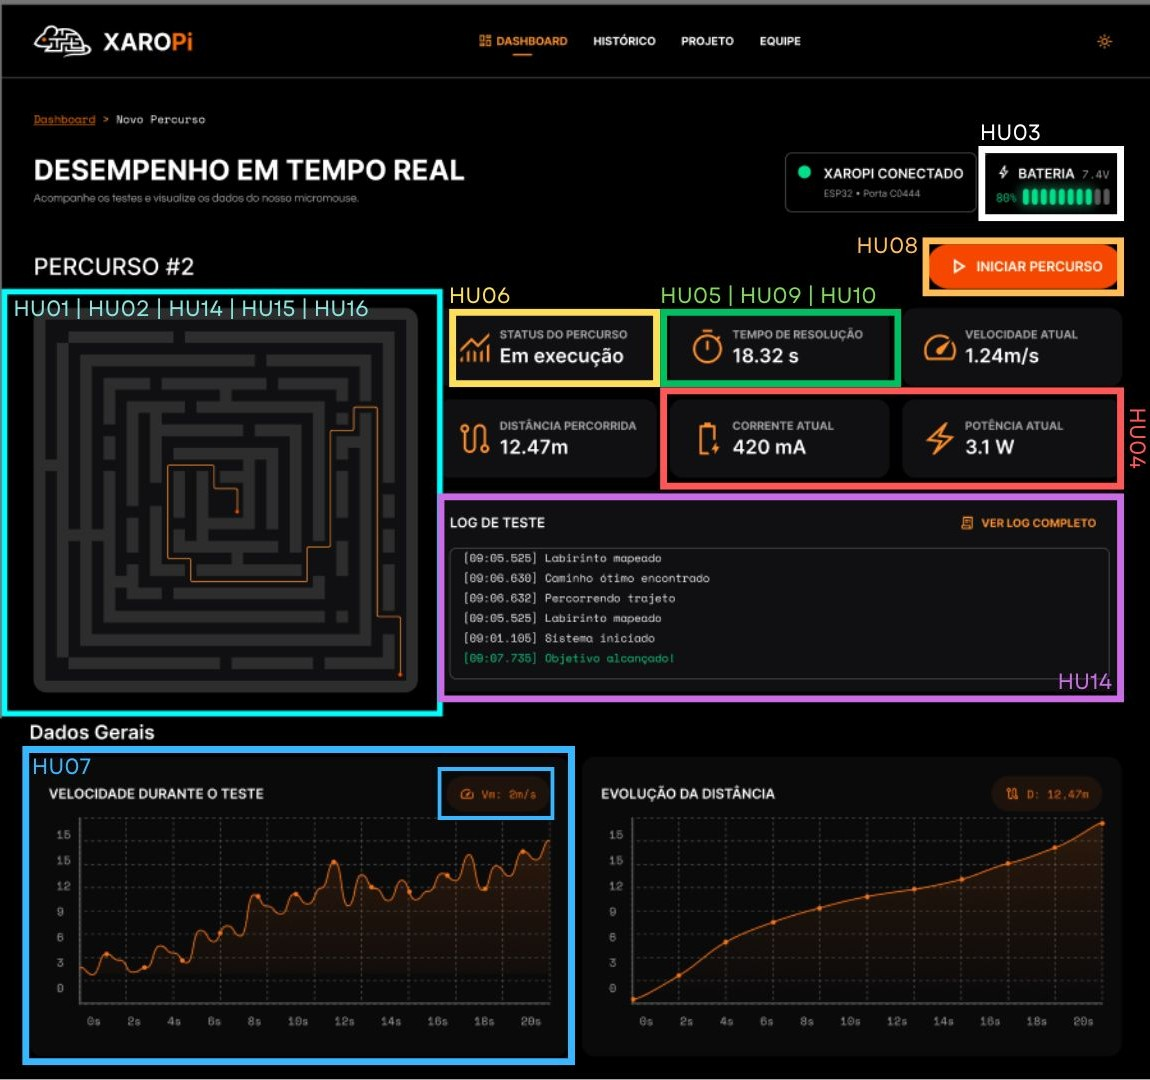
\includegraphics[width=0.65\textwidth]{figuras/software/HUsImplementadas.jpg}
    \caption{HUs implementadas apresentadas no protótipo.}
    \label{fig:hus-implementadas}
\end{figure}

\subsection{Testes unitários do frontend}

Os testes unitários do frontend foram implementados com Vitest. Foram criados testes para os seguintes componentes: badge, battery, bottomBar, breadcrumb, button, card, cell, chart, connection, controlBtn, header, log, maze, modal, tab, table e trace. O código fonte destes testes podem ser acessados em \texttt{src/frontend/src/components/nome\_componente/teste\_componente}.

Os testes verificaram a renderização dos componentes, o recebimento e a exibição correta das propriedades, o comportamento esperado em interações do usuário e a renderização condicional de elementos.

A cobertura dos testes foi analisada utilizando o Vitest. Conforme apresentado na figura \ref{fig:uni_front}, o projeto alcançou 78,37\% de cobertura de instruções e 86,36\% de cobertura de linhas, atendendo ao requisito mínimo de 70\% de cobertura de código-fonte estabelecido pela disciplina.

\begin{figure}[H]
    \centering
    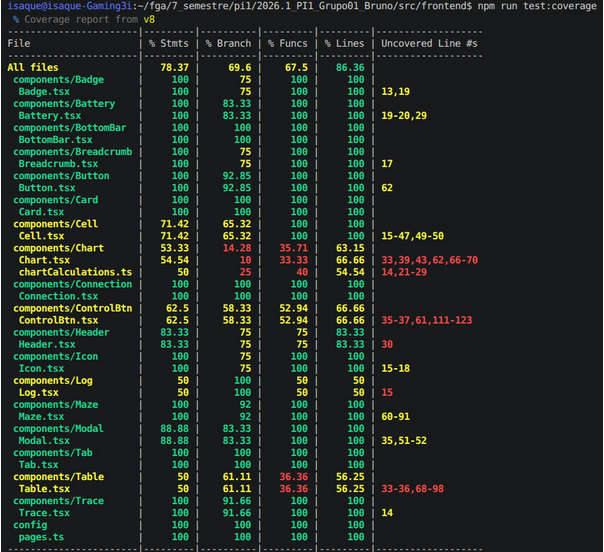
\includegraphics[width=0.7\textwidth]{figuras/software/testes_uni_front.png}
    \captionsetup{font=footnotesize}
    \caption{Relatorio de cobertura dos testes unitários do frontend.}
    \label{fig:uni_front}
\end{figure}

\subsection{Testes unitários do backend}

Os testes unitários do backend foram desenvolvidos com o objetivo de validar o comportamento individual dos serviços, controladores e gateways da aplicação, garantindo que cada módulo funcione corretamente de forma isolada. Para isso, foram utilizados testes automatizados implementados com Jest em conjunto com o módulo de testes do NestJS (\texttt{@nestjs/testing}).

Foram criadas suítes de testes para os principais módulos desenvolvidos. Os módulos contemplados pelos testes unitários são: \texttt{AppController}, \texttt{AppService}, \texttt{FirebaseService} e \texttt{TelemetryGateway}. O código fonte destes testes pode ser acessado em \texttt{src/backend/src}, nos arquivos com sufixo \texttt{.spec.ts} ao lado de cada módulo testado.

Os testes verificaram a inicialização correta dos módulos, o comportamento esperado dos endpoints HTTP, a comunicação via WebSocket com os eventos \texttt{postStart}, \texttt{postNos}, \texttt{postVelBat}, \texttt{postFinish}, \texttt{post\_posicao\_atual} e \texttt{sendcomand}, a integração com o Firebase Realtime Database, o tratamento de erros e o gerenciamento de conexões e desconexões de clientes.

A cobertura dos testes foi analisada utilizando o Jest com a flag \texttt{--coverage}. Conforme apresentado na figura \ref{fig:uni_back}, o projeto alcançou 84,14\% de cobertura de instruções e 84,11\% de cobertura de linhas, superando o requisito mínimo de 70\% de cobertura de código-fonte estabelecido pela disciplina. Os arquivos de configuração de módulos e inicialização da aplicação (\texttt{main.ts}, \texttt{app.module.ts} e \texttt{telemetry.module.ts}) foram excluídos da análise de cobertura por não possuírem lógica de negócio testável. O relatório também permitiu identificar trechos com menor cobertura, como o filtro de exceções WebSocket (\texttt{ws-exception.filter.ts}), servindo como referência para futuras melhorias nas suítes de testes.

\begin{figure}[H]
    \centering
    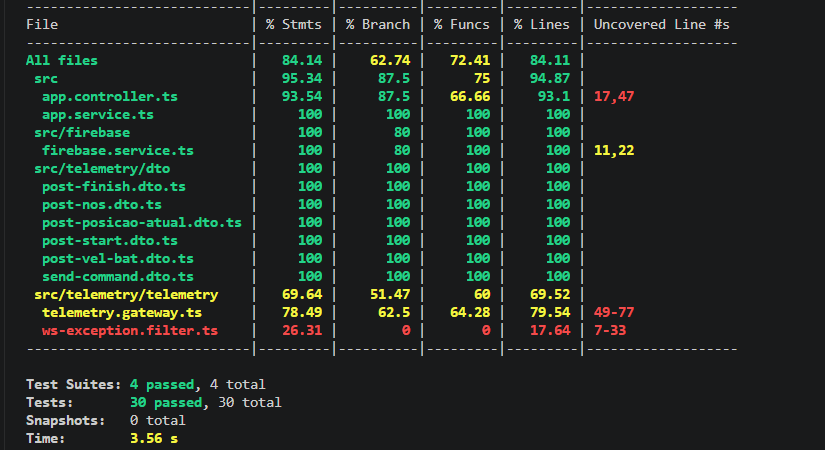
\includegraphics[width=0.7\textwidth]{figuras/software/uni_back.png}
    \captionsetup{font=footnotesize}
    \caption{Relatório de cobertura dos testes unitários do backend.}
    \label{fig:uni_back}
\end{figure}

\subsection{Testes E2E}

Foram implementados testes end-to-end utilizando Cypress com base nos roteiros de testes funcionais definidos na primeira entrega do projeto. Até o momento, foi possível implementar os casos de teste do CT1 ao CT5. O código fonte destes testes pode ser acessado em \texttt{src/frontend/src/cypress/e2e}. 

Os testes tiveram resultado positivo nos cenários CT1, CT2, CT4 e CT5. O CT3 apresentou falha por não exibir o resultado concluído na tela ao finalizar o percurso com sucesso, entretanto envia os dados corretamente para o banco.

\subsubsection{Caso de Teste 04 (CT4): Consulta de Histórico}
O CT4 tem como objetivo validar o carregamento e a renderização da tabela de histórico de percursos. O teste automatizado navega até a rota correspondente, intercepta a requisição da API e verifica se os registros antigos estão sendo listados sem perda de informação.

\begin{figure}[H]
    \centering
    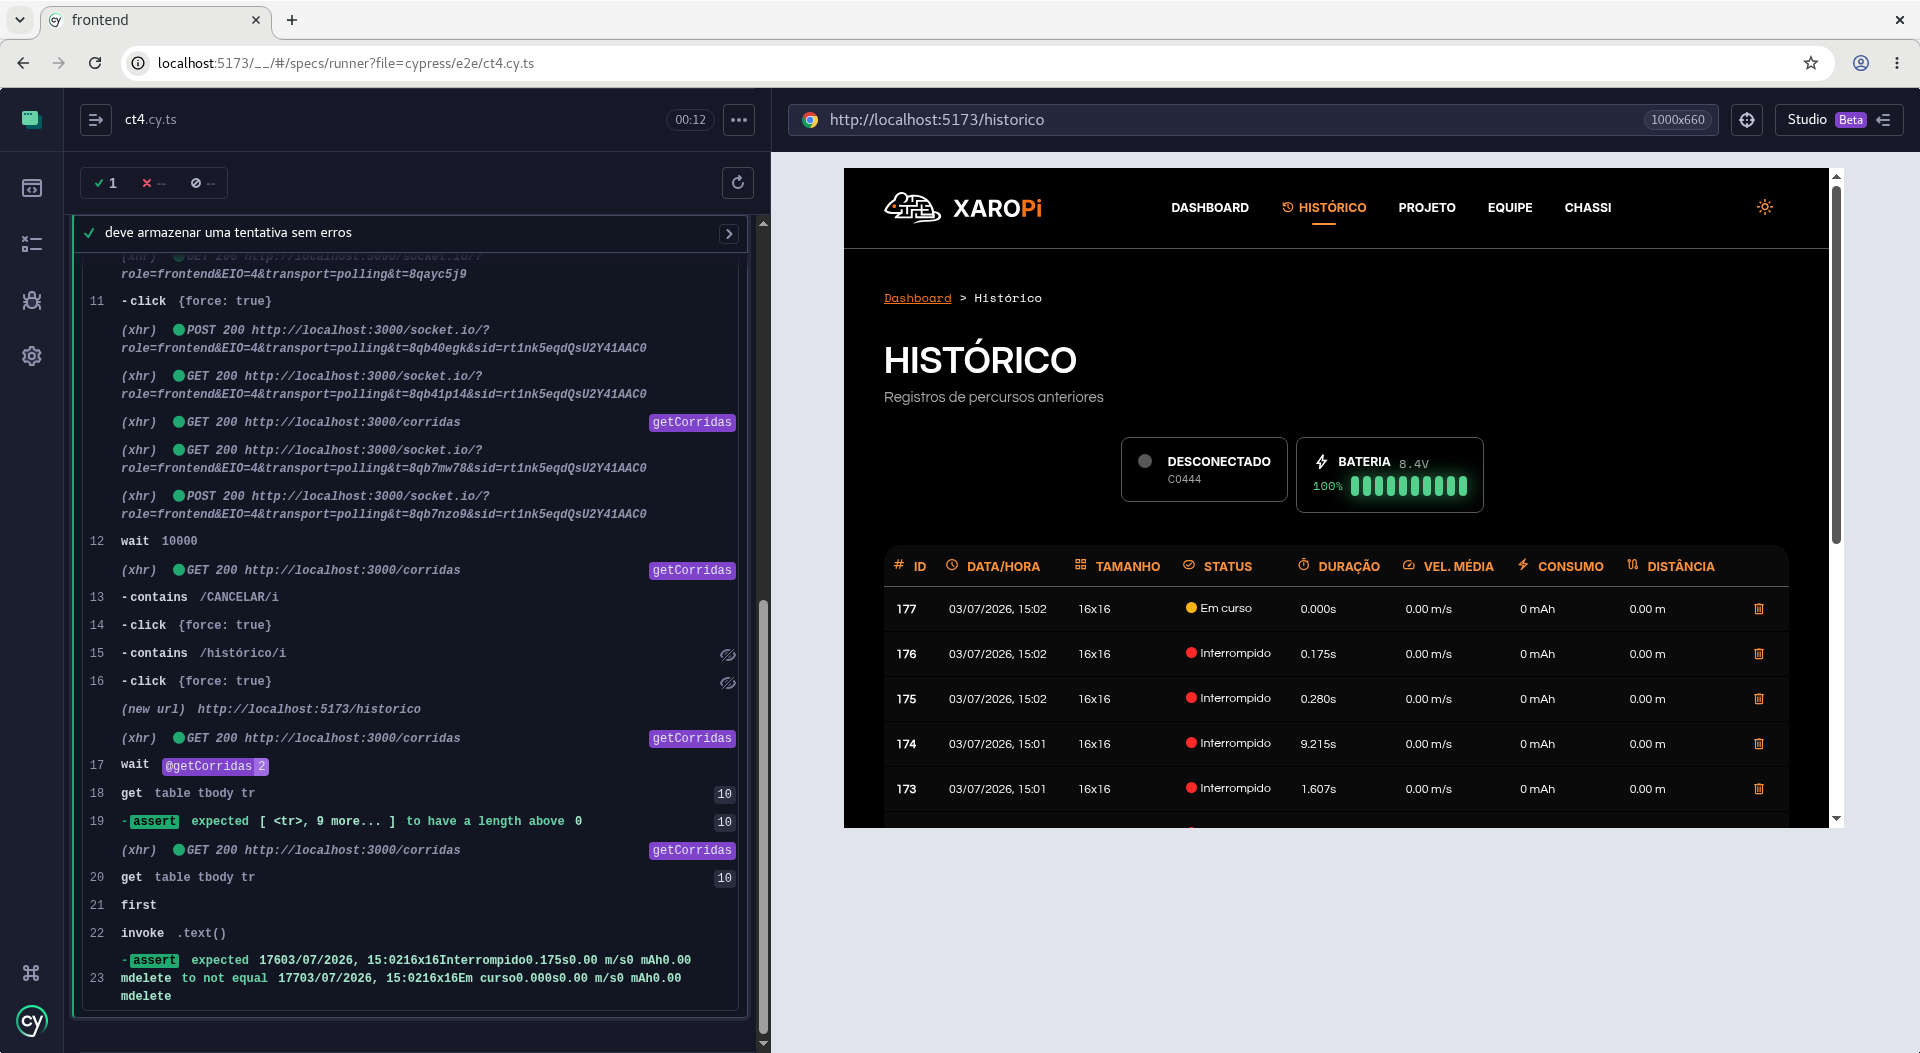
\includegraphics[width=0.9\textwidth]{figuras/software/ct4_cypress.png} 
    \caption{Execução do Caso de Teste 04 aprovada no Cypress Runner.}
    \label{fig:ct4_cypress}
\end{figure}

\subsubsection{Caso de Teste 05 (CT5): Visualização de Percurso Específico}
O CT5 avança no fluxo do histórico, testando a funcionalidade de inspecionar uma corrida passada. O Cypress valida se, ao acessar a página de detalhes, os dados gerais do percurso, bem como os gráficos de telemetria, são exibidos de forma correta e síncrona.

\begin{figure}[H]
    \centering
    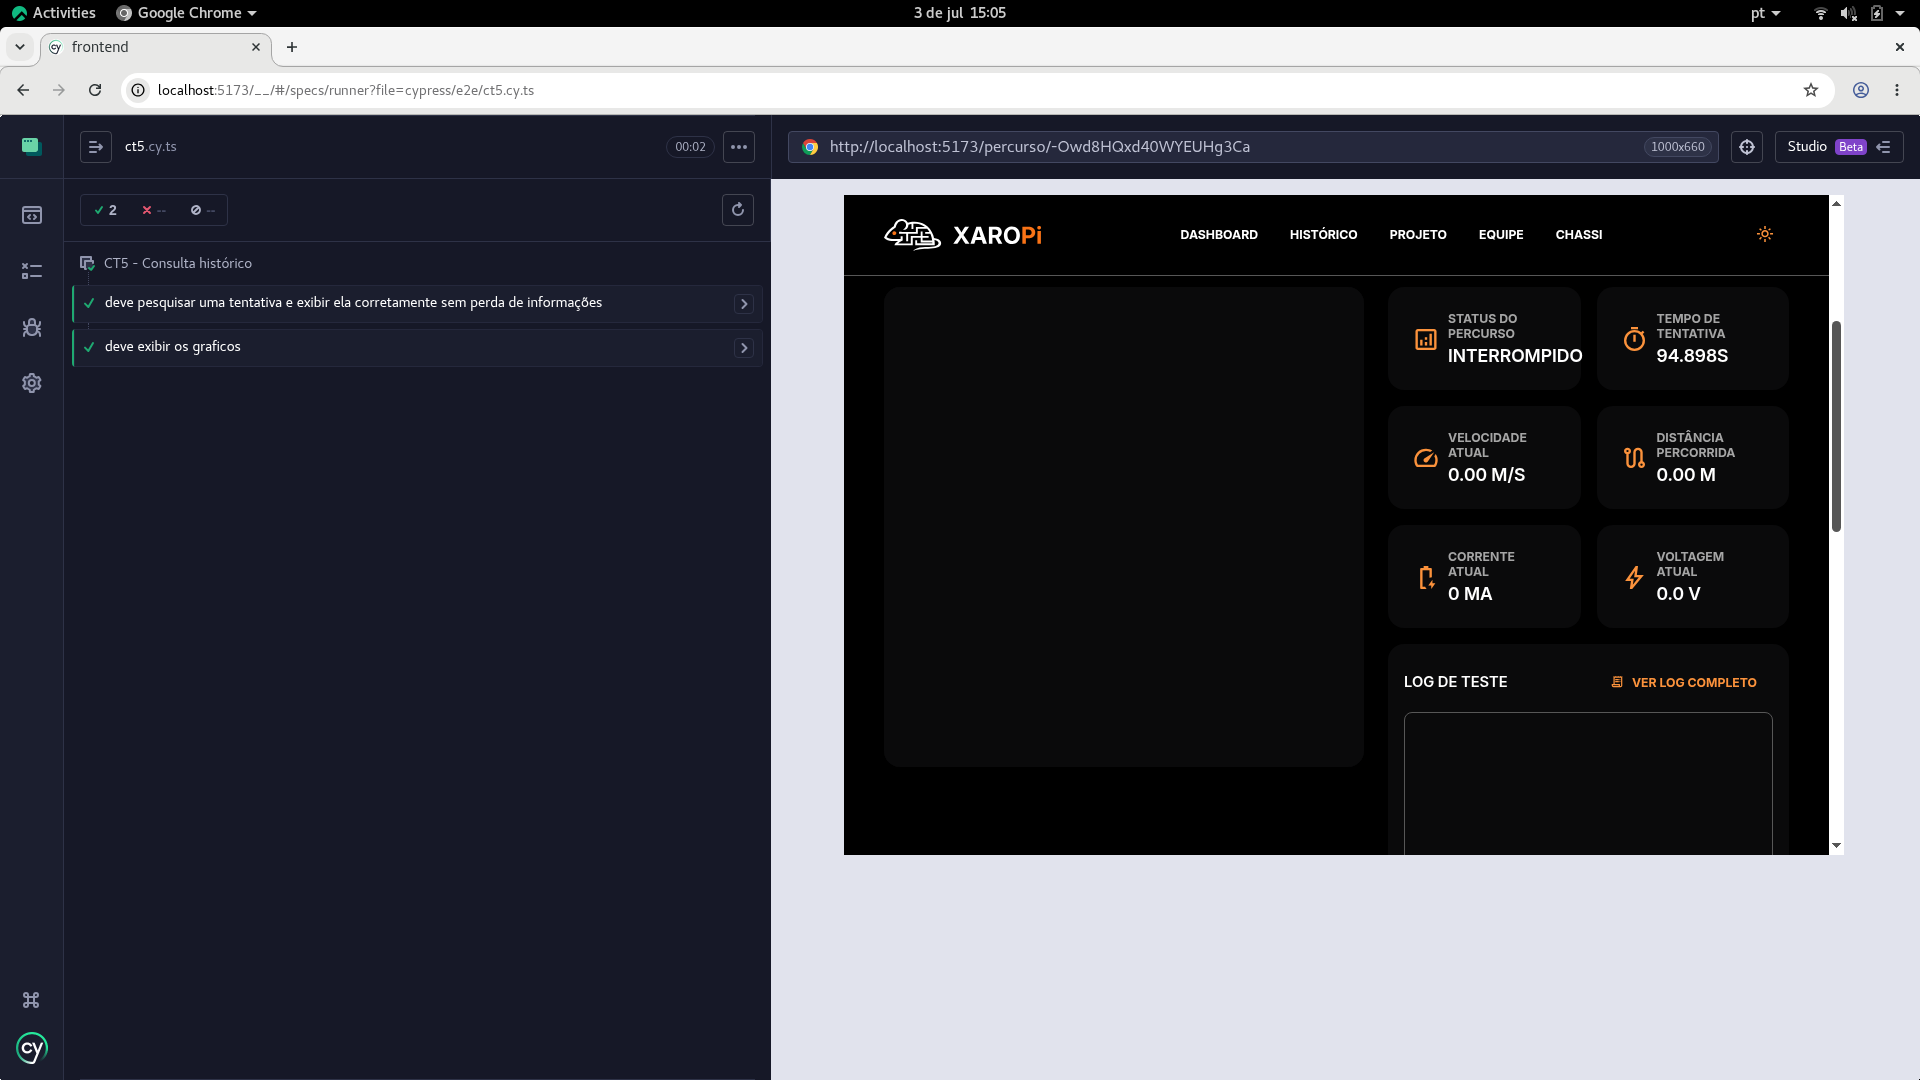
\includegraphics[width=0.9\textwidth]{figuras/software/ct5_cypress.png}
    \caption{Execução do Caso de Teste 05 aprovada no Cypress Runner.}
    \label{fig:ct5_cypress}
\end{figure}

\subsection{Testes de integração}

Os testes de integração tiveram como foco principal validar os \textit{endpoints} da API e sua correta orquestração com a camada de serviços responsáveis pela comunicação e persistência de dados no Firebase Realtime Database.

Para a realização das chamadas, utilizou-se a biblioteca \textit{Supertest}, que simula requisições HTTP e avalia os códigos de status e corpos de resposta. A suíte de testes contemplou o fluxo completo de gerenciamento de corridas e telemetria:

\begin{itemize}
    \item \textbf{GET / (Healthcheck):} Validação da disponibilidade e tempo de resposta da API.
    \item \textbf{POST /telemetria:} Validação do recebimento do \textit{payload} estruturado pelo robô e do acionamento do serviço de salvamento.
    \item \textbf{GET /corridas:} Validação da recuperação, estruturação e formatação dos dados provindos do banco de dados.
    \item \textbf{DELETE /corridas/:id:} Validação da rotina de remoção de registros.
\end{itemize}

Durante a validação, devido a restrições rigorosas de rede no ambiente de desenvolvimento Linux (isolamento provocado por contêineres Flatpak), a conexão externa direta aos servidores do Google Cloud sofreu bloqueios operacionais, falhas de \textit{timeout} e \textit{Gaxios Error}. 

Para contornar essa limitação de infraestrutura sem comprometer a validação da arquitetura, aplicou-se a técnica de \textit{Provider Override} suportada nativamente pelo NestJS. Os serviços de conexão direta, \texttt{FirebaseService} e \texttt{AppService}, foram interceptados e mockados com respostas controladas. 

Essa abordagem atesta que os controladores, as rotas e o sistema de injeção de dependências estão perfeitamente integrados e capazes de processar os dados adequadamente até a fronteira final com o banco de dados. Como ilustrado na figura \ref{fig:integracao_back}, a bateria de testes foi aprovada com sucesso.

\begin{figure}[H]
    \centering
    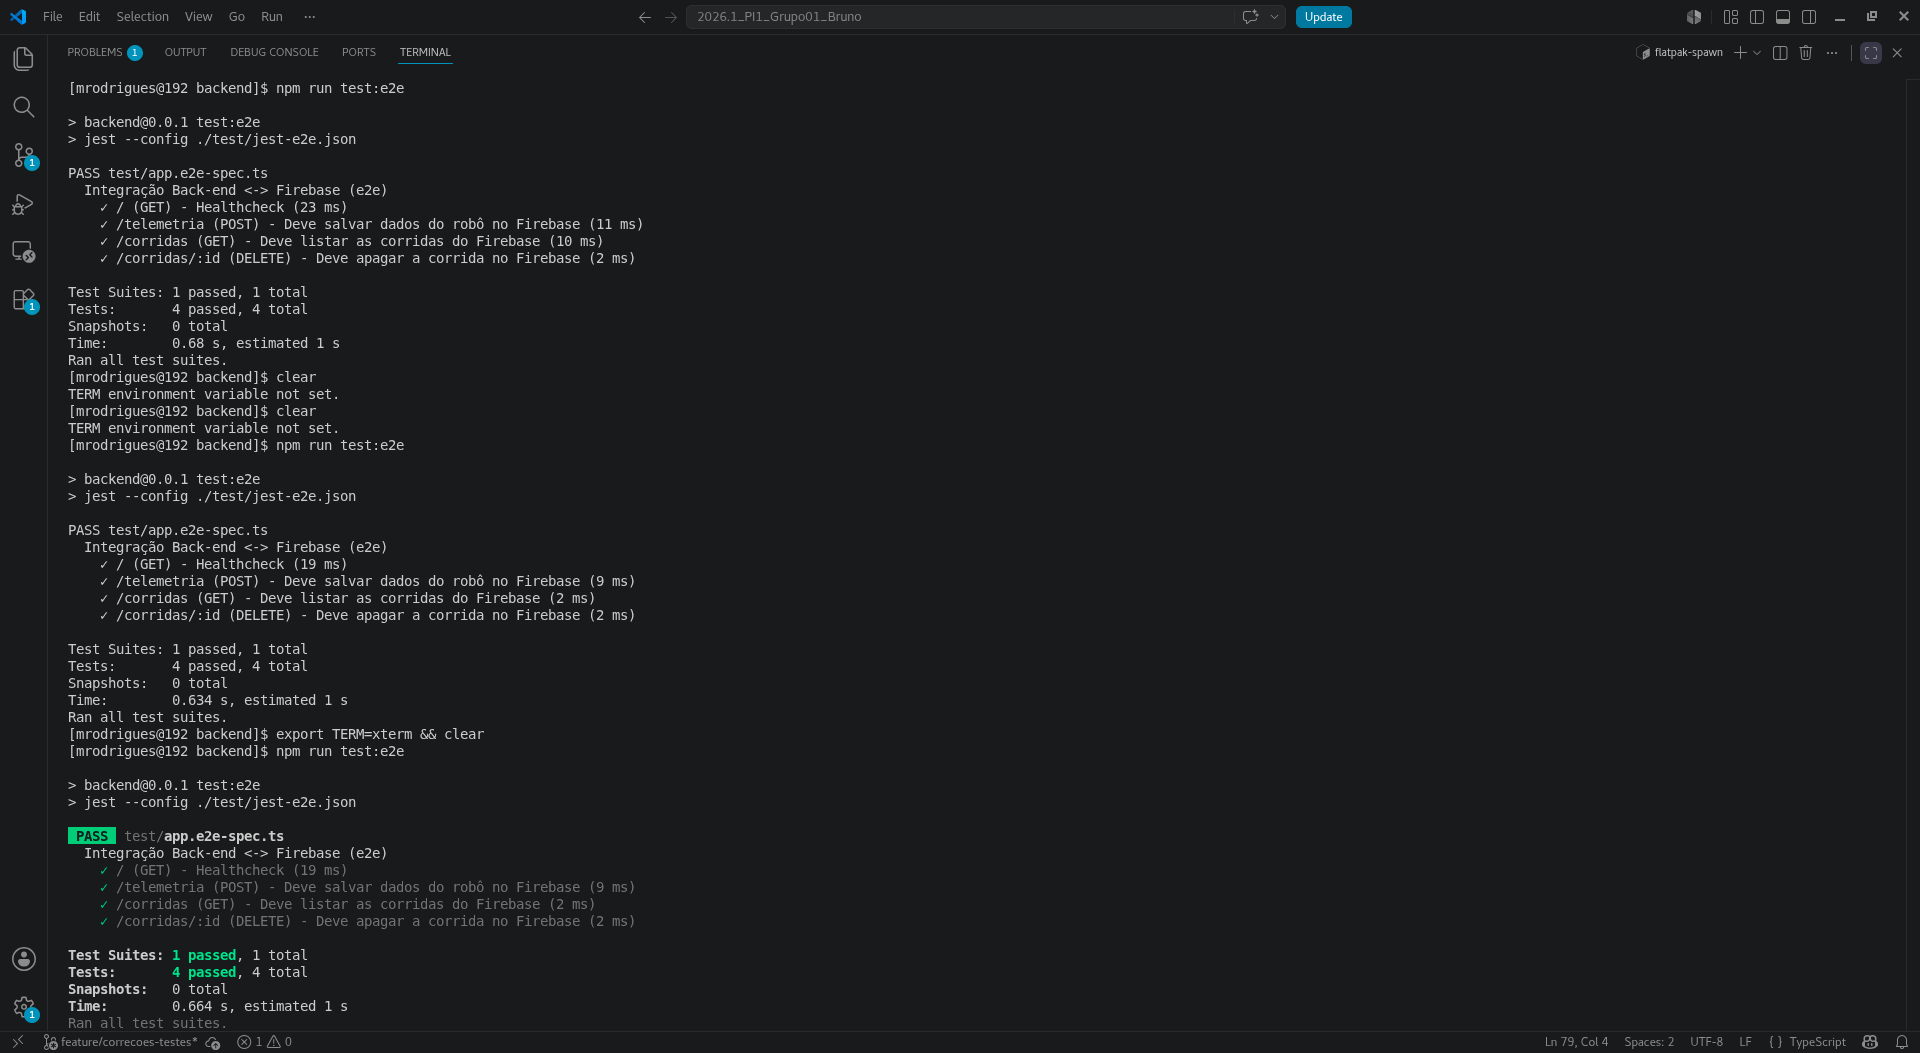
\includegraphics[width=0.7\textwidth]{figuras/software/testeIntegracao.png} 
    \captionsetup{font=footnotesize}
    \caption{Relatório de aprovação dos testes de integração da API (Supertest).}
    \label{fig:integracao_back}
\end{figure}

Além dos testes via \textit{Supertest} sobre os endpoints REST, foi conduzido um teste de integração da camada de comunicação em tempo real, responsável pela troca de telemetria entre o firmware do robô e o backend. Diferentemente dos testes anteriores, essa validação foi executada com o hardware físico conectado à rede \textit{Access Point} da ESP32, permitindo observar o comportamento real do protocolo \textit{Socket.IO} nas duas pontas da comunicação.

Do lado do servidor, o \texttt{TelemetryGateway} foi instrumentado com um sistema de \textit{logging} detalhado, capaz de registrar cada etapa do ciclo de vida da conexão: o recebimento do \textit{handshake} (incluindo parâmetros de \textit{query} como \texttt{role} e endereço IP de origem), a identificação do cliente como firmware, o envio do evento de confirmação \texttt{firmware\_ack} e a propagação do evento \texttt{firmware\_status} para a sala dos clientes \textit{frontend}. Como ilustrado na figura \ref{fig:integracao_ws_backend}, o servidor inicializa corretamente todos os \textit{gateways} e rotas antes de identificar e confirmar a conexão da placa (\texttt{socket.id=VadC7H4PxRelRcUtAAAB}), validando o correto funcionamento da inicialização da aplicação NestJS e do módulo de \textit{WebSockets}.

Do lado do firmware, o monitor serial da ESP32 confirma a recepção do evento de confirmação enviado pelo backend, registrando a mensagem \texttt{[IO] CONECTADO!} seguida do \textit{payload} \texttt{firmware\_ack} com o \textit{status} \texttt{"conectado"} e o respectivo \textit{timestamp}, conforme apresentado na figura \ref{fig:integracao_ws_firmware}. Esse resultado comprova que o protocolo de conexão implementado é bidirecional e íntegro: o backend reconhece e confirma a placa, e a placa recebe e interpreta corretamente essa confirmação, validando de ponta a ponta a integração entre o firmware embarcado e o serviço de telemetria em tempo real.

\begin{figure}[H]figuras/testeIntegracaoWebSocketFirmware.png
    \centering
    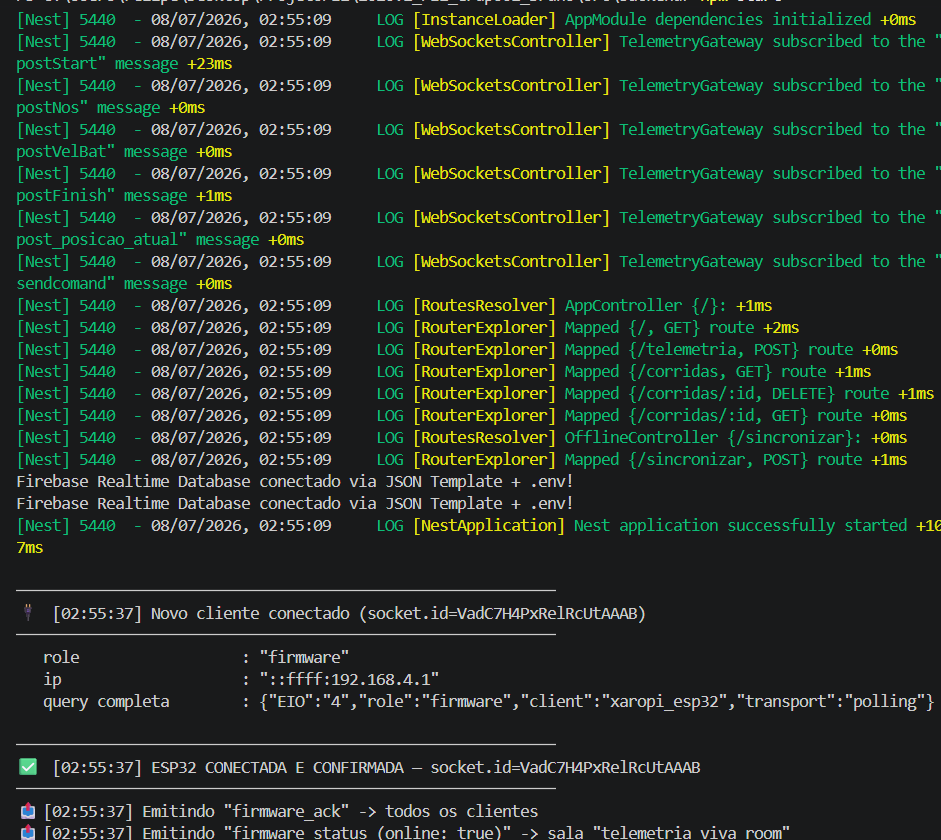
\includegraphics[width=0.7\textwidth]{figuras/testeIntegracaoWebSocketFirmware.png} 
    \captionsetup{font=footnotesize}
    \caption{Logs do backend NestJS durante a inicialização e a conexão da ESP32 via WebSocket.}
    \label{fig:integracao_ws_backend}
\end{figure}

\begin{figure}[H]
    \centering
    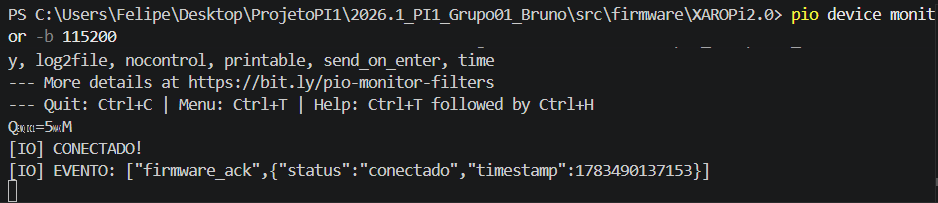
\includegraphics[width=0.7\textwidth]{figuras/testeIntegracaoWebSocketBackend.png} 
    \captionsetup{font=footnotesize}
    \caption{Monitor serial da ESP32 confirmando o recebimento do evento \texttt{firmware\_ack}.}
    \label{fig:integracao_ws_firmware}
\end{figure}